\xchapter{Revisão Bibliográfica}{}



\section{Engenharia de Software}

A Engenharia de Software é uma disciplina fundamental para a construção sistemática, disciplinada e mensurável de sistemas computacionais. De acordo com \citeonline{sommerville2011}, a ES não se restringe à atividade de programação, mas abrange todas as etapas do ciclo de vida do software, desde a especificação inicial até a manutenção de sistemas em operação. Seu objetivo central é assegurar que os sistemas sejam desenvolvidos de maneira confiável, econômica e em conformidade com as necessidades dos usuários.

Ademais, \citeonline{pressman2016} complementa essa visão ao descrever a ES como uma tecnologia alicerçada em camadas. Em sua base está o compromisso contínuo com a qualidade, sobre o qual se apoiam o processo, os métodos e as ferramentas. O processo define as atividades e práticas que orientam o desenvolvimento; os métodos oferecem o suporte técnico para análise, projeto, implementação e testes; e as ferramentas fornecem automação para aumentar a produtividade e a consistência.

Nesse sentido, ambos os autores convergem ao destacar que a Engenharia de Software é uma prática sócio-técnica, que integra dimensões técnicas, humanas e organizacionais. Isso implica reconhecer que fatores como comunicação eficaz, gerenciamento de riscos, colaboração entre equipes e adaptabilidade são tão cruciais quanto as próprias técnicas de desenvolvimento.

Sob essa ótica, este trabalho se fundamenta nos princípios da Engenharia de Software para investigar a aplicação de \textit{Large Language Models}  no apoio à análise de conformidade entre requisitos e código. A pesquisa propõe-se a conectar os desafios clássicos da área, especialmente a rastreabilidade semântica entre especificações em linguagem natural e suas implementações com as oportunidades oferecidas por tecnologias emergentes, buscando soluções mais eficientes e automatizadas.

\subsection{Engenharia de Requisitos}

A Engenharia de Requisitos é reconhecida como uma das atividades centrais da Engenharia de Software, sendo responsável por estabelecer a base sobre a qual o sistema será desenvolvido. Sua finalidade é transformar as necessidades dos \textit{stakeholders} em especificações compreensíveis, consistentes e verificáveis, criando um elo entre os objetivos de negócio e a solução técnica. Como destaca \citeonline{sommerville2011}, a Engenharia de Requisitos é um processo iterativo que envolve identificar os serviços que o sistema deve oferecer e as restrições que condicionam seu funcionamento.

A literatura aponta que falhas nessa etapa representam uma das principais causas de insucesso em projetos de software. \citeonline{pressman2016} enfatiza que compreender o que deve ser construído é, frequentemente, mais desafiador do que a própria construção, pois clientes e usuários raramente possuem uma visão completa de suas necessidades ou as expressam de forma inequívoca. Ademais, os requisitos são naturalmente voláteis, sofrendo alterações ao longo do projeto. Desse modo, a Engenharia de Requisitos deve ser entendida como um processo contínuo de comunicação, análise e validação.

Do ponto de vista processual, a Engenharia de Requisitos compreende um conjunto de atividades integradas. Inicia-se pela concepção, que define o escopo preliminar do problema. Segue-se para a elicitação, que consiste na coleta estruturada de informações por meio de técnicas como entrevistas, prototipação e análise documental. A fase de análise e elaboração busca refinar os dados obtidos, identificando inconsistências e ambiguidades. Dada a diversidade de interesses, a negociação torna-se indispensável para conciliar demandas conflitantes dentro das restrições do projeto.

Uma vez definidas as prioridades, procede-se à especificação, formalizada em documentos como a \textit{Software Requirements Specification} (SRS), que registram requisitos funcionais e não funcionais. A etapa seguinte, a validação, verifica se as especificações refletem as necessidades dos \textit{stakeholders} e se são completas e testáveis, utilizando técnicas como revisões e simulações. Por fim, a gestão de requisitos garante o acompanhamento das mudanças ao longo do ciclo de vida, mantendo vínculos claros entre requisitos, implementações e testes para preservar a rastreabilidade.

O Guia PMBOK \cite{pmi2008}, por sua vez, insere a Engenharia de Requisitos no contexto do gerenciamento do escopo do projeto, destacando que cada necessidade deve ser documentada e vinculada a entregáveis mensuráveis. A rastreabilidade, nesse sentido, é um mecanismo essencial que assegura a correta implementação e verificação dos requisitos, promovendo o alinhamento entre planejamento, execução e controle.

Assim, a Engenharia de Requisitos não se limita a uma etapa preliminar de coleta de informações, mas constitui um processo contínuo e estruturado, que articula comunicação entre \textit{stakeholders}, documentação formal, validação sistemática e gestão de mudanças. Ao desempenhar esse papel central, garante que os sistemas de software sejam construídos de forma a atender às expectativas dos usuários, respeitar restrições operacionais e oferecer qualidade consistente ao longo de seu ciclo de vida.

\subsection{Gerenciamento de Prazos e Custos}

O gerenciamento de prazos e custos constitui uma das áreas mais sensíveis da Engenharia de Software, dada a natureza abstrata do produto e a volatilidade dos requisitos. A ausência de elementos físicos tangíveis, somada às dificuldades de mensuração do esforço intelectual, torna a previsão de tempo e orçamento uma atividade inerentemente incerta e sujeita a desvios.

Segundo \citeonline{sommerville2011}, abordagens de planejamento rígido apresentam limitações em projetos de software, especialmente em contextos onde mudanças são inevitáveis. Nesses casos, modelos iterativos e incrementais, que permitem reavaliações contínuas, proporcionam maior capacidade de resposta a imprevistos. O autor destaca, ainda, a importância do replanejamento constante e do envolvimento dos \textit{stakeholders} para garantir o alinhamento entre expectativas e entregáveis.

Do ponto de vista operacional, o planejamento envolve a definição de atividades, a estimativa de esforço, a alocação de recursos e o estabelecimento de marcos de controle. \citeonline{pressman2016} enfatiza que a precisão das estimativas depende da maturidade organizacional e da disponibilidade de dados históricos. Em ambientes estruturados, técnicas como a Análise de Pontos de Função e o modelo COCOMO (\textit{Constructive Cost Model}) são utilizadas para fornecer estimativas quantitativas, permitindo simular cenários de custo e cronograma com base em parâmetros como complexidade e capacidade da equipe.

A comunicação eficaz também é um pilar deste processo. Conforme argumenta \citeonline{sommerville2011}, falhas na comunicação figuram entre as principais causas de atrasos e estouros orçamentários. A revisão periódica dos planos, o registro transparente de mudanças e a gestão ativa das expectativas são, portanto, cruciais para a manutenção do controle do projeto.

Nesse contexto, a conexão entre a conformidade de requisitos e o gerenciamento de prazos e custos torna-se evidente. O retrabalho, decorrente de funcionalidades implementadas em desacordo com o especificado, é um dos principais fatores de erosão de cronogramas e orçamentos. Portanto, a investigação de ferramentas que automatizam a verificação da conformidade, como proposto neste trabalho, representa uma abordagem proativa para mitigar riscos financeiros e temporais, reduzindo a incidência de correções tardias e onerosas.

\subsection{Qualidade de Software}

A qualidade de software é o resultado de um processo que integra planejamento, definição de métricas, verificação contínua e validação sistemática de requisitos. De acordo com \citeonline{sommerville2011}, a qualidade não se restringe ao produto final, mas depende fundamentalmente do processo adotado para desenvolvê-lo. De forma complementar, \citeonline{pressman2016} argumenta que a qualidade deve ser construída ao longo de todo o ciclo de vida e avaliada por meio de medições objetivas, em vez de depender de inspeções pontuais.


O estabelecimento de métricas é um processo colaborativo. O Guia PMBOK \cite{pmi2008} aponta que a definição dos parâmetros de avaliação é uma responsabilidade compartilhada entre gestores, \textit{stakeholders} e desenvolvedores. Em projetos de maior porte, equipes de \textit{Quality Assurance} (QA) atuam de forma independente para assegurar a imparcialidade na validação. Em contextos menores, esse papel pode ser desempenhado pelo time de desenvolvimento,  embora \citeonline{sommerville2011} alerte que a falta de independência pode comprometer a objetividade da avaliação.

A validação da implementação de um requisito depende, primeiramente, da definição de critérios de aceitação claros, que descrevem em que condições a funcionalidade pode ser considerada concluída. Esses critérios são transformados em casos de teste, os quais simulam tanto cenários de uso esperados quanto situações de exceção.\citeonline{pressman2016} destaca que a determinação da quantidade de cenários de teste deve estar diretamente relacionada à complexidade do requisito: funcionalidades críticas, com múltiplas entradas ou impacto na segurança, exigem uma cobertura mais extensa do que funcionalidades simples e de baixo risco. \citeonline{sommerville2011} acrescenta que, em muitos casos, os testes devem abranger não apenas requisitos funcionais verificando se a função solicitada foi implementada corretamente, mas também requisitos não funcionais, como desempenho, confiabilidade e usabilidade, cuja validação demanda métricas específicas.

A medição da qualidade resulta, portanto, da combinação de diferentes perspectivas. Por um lado, existem métricas quantitativas, como a cobertura de requisitos (proporção de requisitos associados a testes), a densidade de defeitos (número de falhas encontradas por unidade de artefato) e o esforço médio para corrigir erros, amplamente discutidas por \citeonline{pressman2016}. Por outro lado, existem aspectos qualitativos, como a clareza da documentação, a consistência de interfaces e a facilidade de manutenção, que, ainda segundo Sommerville, exigem inspeções estruturadas e o julgamento de especialistas.

O Guia PMBOK \cite{pmi2008} enfatiza que tais processos de avaliação devem ser acompanhados de forma contínua, envolvendo tanto a prevenção quanto a correção de falhas. A prevenção é garantida pelo planejamento da qualidade, quando se definem padrões, métricas e critérios de aceitação, já a correção ocorre nos processos de controle, quando os resultados de testes e inspeções são comparados com os padrões estabelecidos e são adotadas ações corretivas em caso de desvios. Assim, a definição de métricas, a escolha dos testes e a determinação da quantidade de cenários não são decisões arbitrárias, mas decorrem de um processo de gestão da qualidade que envolve múltiplos agentes, desde o cliente até a equipe técnica, e que se apoia em práticas consolidadas de engenharia de software.

Em síntese, a validação da implementação de um requisito não se limita a confirmar a presença de código correspondente, mas exige que sejam definidos critérios de aceitação verificáveis, transformados em cenários de teste, avaliados por meio de métricas objetivas e complementados por revisões independentes. A qualidade, portanto, emerge de um processo coletivo e interativo, que combina prevenção, medição e melhoria contínua, garantindo que o software entregue esteja não apenas em conformidade com as especificações, mas também adequado ao uso e sustentável em longo prazo.

\subsection{Fatores Críticos em Projetos de Software}

O êxito de projetos de software transcende a aplicação de técnicas e ferramentas, dependendo de um espectro de fatores organizacionais, humanos e gerenciais. \citeonline{sommerville2011} argumenta que falhas de comunicação estão entre as principais causas de insucesso, pois comprometem o alinhamento de expectativas e geram ambiguidades nos requisitos. O autor também destaca a ausência de um gerenciamento de riscos estruturado como um fator que reduz a resiliência do projeto.

O êxito de projetos de software não depende exclusivamente da aplicação de técnicas e ferramentas de desenvolvimento, mas também de uma ampla gama de fatores organizacionais, humanos e gerenciais. \citeonline{sommerville2011} argumenta que falhas de comunicação entre os membros da equipe e os \textit{stakeholders} figuram entre as principais causas de insucesso em projetos de software, uma vez que comprometem o alinhamento de expectativas, dificultam a tomada de decisões e favorecem o surgimento de ambiguidade nos requisitos. Além disso, o autor destaca que a ausência de práticas estruturadas de gerenciamento de riscos reduz a capacidade do projeto de responder adequadamente a imprevistos, afetando diretamente sua resiliência e previsibilidade.

Complementarmente, \citeonline{pressman2016} enfatiza a importância da motivação e da capacitação da equipe como elementos essenciais. Times engajados e tecnicamente preparados respondem com maior eficiência a pressões de prazo, escopo e desafios técnicos. O autor ressalta, ainda, que arquiteturas modulares e documentação consistente favorecem a sustentabilidade do software ao longo de seu ciclo de vida.

Outro aspecto relevante é a gestão do conhecimento. Ambientes que promovem a troca de experiências e a retroalimentação de processos apresentam melhores índices de produtividade e qualidade, especialmente em cenários de alta incerteza. Dessa forma, os fatores críticos de sucesso resultam da integração equilibrada entre pessoas, processos e tecnologia, exigindo uma abordagem holística do desenvolvimento.

Dessa forma, os fatores críticos de sucesso em projetos de software podem ser compreendidos como resultado da integração equilibrada entre pessoas, processos e tecnologia. Tal integração pressupõe uma abordagem holística do desenvolvimento de software, na qual aspectos técnicos não são tratados isoladamente, mas articulados com práticas gerenciais, estratégias de comunicação, definição clara de papéis e investimento contínuo em capacitação.

Em síntese, o sucesso de um projeto não é determinado apenas pela adoção de boas práticas técnicas, mas pela capacidade da organização de estruturar um ecossistema de desenvolvimento que favoreça a adaptação, o comprometimento coletivo e a gestão proativa dos fatores críticos que impactam diretamente o desempenho e a entrega de valor do software. Contudo, mesmo em ambientes bem estruturados, subsiste um desafio persistente: garantir que os requisitos formalmente definidos sejam de fato corretamente implementados, preservando sua intenção original ao longo do ciclo de vida do software. 

Ferramentas tradicionais, como linters e analisadores estáticos, embora eficazes na detecção de erros sintáticos e estruturais no código-fonte, não possuem mecanismos capazes de interpretar a semântica contida em documentos de requisitos escritos em linguagem natural. Essa limitação compromete sua eficácia na verificação da conformidade entre especificações e implementações, especialmente em contextos complexos e sujeitos a variações terminológicas. É precisamente nessa lacuna que os LLMs se inserem como uma inovação promissora. Dotados de mecanismos avançados de representação contextual e capacidade de correlacionar textos descritivos com estruturas de código, esses modelos inauguram uma nova classe de ferramentas capazes de realizar análises semânticas mais profundas e alinhadas ao domínio da Engenharia de Requisitos. Assim, ao incorporar LLMs ao processo de verificação de conformidade, este trabalho busca explorar seu potencial para aprimorar a rastreabilidade, mitigar ambiguidades e reduzir o retrabalho decorrente de interpretações incorretas ou incompletas dos requisitos.


\section{Aprendizado de Máquina}

O Aprendizado de Máquina (AM) é caracterizado por ser a área voltada ao desenvolvimento de algoritmos capazes de identificar padrões em dados e, a partir deles, realizar previsões ou decisões. Segundo \citeonline{jelodar2025}, essa abordagem tem se consolidado como fundamental para tarefas de análise de código, processamento de linguagem natural e suporte a sistemas de recomendação, dado seu potencial de generalização a partir de grandes volumes de dados.

Tradicionalmente, o AM é dividido em três paradigmas: aprendizado supervisionado, não supervisionado e por reforço. O primeiro baseia-se em conjuntos de dados rotulados, permitindo que o modelo aprenda a relação entre entradas e saídas conhecidas. Em contrapartida, o aprendizado não supervisionado busca descobrir estruturas ocultas ou agrupamentos em dados não rotulados, sendo amplamente aplicado em técnicas de clusterização e redução de dimensionalidade. O aprendizado por reforço, por sua vez, concentra-se na interação de um agente com um ambiente, onde decisões são ajustadas com base em recompensas ou penalidades recebidas.

Nesse contexto, no campo do Processamento de Linguagem Natural, o Aprendizado de Máquina tem desempenhado papel essencial para a evolução de modelos cada vez mais robustos. O advento da arquitetura Transformer, proposta por \citeonline{vaswani2017}, representou um marco nesse cenário, ao introduzir mecanismos de atenção capazes de capturar dependências de longo alcance em sequências textuais. Essa inovação viabilizou a criação dos LLMs, que combinam técnicas de aprendizado profundo com grandes volumes de dados textuais para realizar tarefas como tradução automática, sumarização, análise de sentimentos e verificação semântica.

\subsection{Redes Neurais e Deep Learning}

As Redes Neurais Artificiais (RNAs) constituem uma classe de algoritmos de aprendizado de máquina inspirada na estrutura e no funcionamento do cérebro humano \citeonline{choi2020}. Essencialmente, uma rede neural é uma coleção de neurônios e conexões entre eles. Um neurônio pode ser entendido como uma função matemática que recebe um conjunto de entradas, realiza uma operação sobre elas e produz uma única saída. As conexões funcionam como canais que ligam a saída de um neurônio à entrada de outro, e cada conexão possui um peso que determina a força ou a importância do sinal transmitido. É através do ajuste desses pesos que a rede aprende.

Uma das arquiteturas fundamentais de uma rede neural é o Perceptron, introduzido por Rosenblatt (1958) como um modelo probabilístico para armazenamento e organização de informação no cérebro. O Perceptron é um algoritmo que recebe um conjunto de entradas (features) e busca encontrar uma linha, plano ou hiperplano capaz de separar os dados em diferentes classes \citeonline{asimov2017}. Quando múltiplos perceptrons são interligados em camadas, a estrutura passa a ser denominada Rede Neural Artificial ou Perceptron de Múltiplas Camadas (MLP).

Em uma arquitetura \textit{Feedforward} (FFNN), os neurônios são organizados em uma camada de entrada, uma ou mais camadas ocultas e uma camada de saída. A informação flui estritamente em uma direção, da entrada para a saída, sem ciclos ou retroalimentação. Para que a rede possa aprender padrões não lineares complexos, os neurônios nas camadas ocultas e de saída aplicam uma função de ativação não linear, como a sigmoide ou a Unidade Linear Retificada (ReLU), à soma ponderada de suas entradas \citeonline{choi2020}.

Esse processo de treinamento é tipicamente realizado por meio do algoritmo de \textit{backpropagation}. A rede recebe um conjunto de dados de treinamento e, para cada exemplo, sua saída é comparada com a saída desejada (rótulo) através de uma função de perda (ou custo). O algoritmo então calcula o gradiente dessa função de perda em relação a cada peso na rede e ajusta os pesos na direção que minimiza o erro. Esse processo é repetido iterativamente para todo o conjunto de dados.

O conceito de Aprendizado Profundo (\textit{Deep Learning}) refere-se ao uso de redes neurais com um número substancial de camadas ocultas, frequentemente chamadas de Redes Neurais Profundas (DNNs). Essa profundidade permite que a rede aprenda uma hierarquia de características, onde as camadas iniciais detectam padrões simples e as camadas subsequentes combinam essas características para reconhecer conceitos mais complexos e abstratos. Um dos desafios históricos do aprendizado profundo foi a dificuldade de treinar redes com muitas camadas. Para contornar essa dificuldade, uma solução que impulsionou a área foi o pré-treinamento guloso camada a camada (\textit{greedy layer-wise pre-training}), onde cada camada é treinada de forma não supervisionada para aprender uma representação da saída da camada anterior. Após o pré-treinamento de todas as camadas, a rede inteira passa por um ajuste fino supervisionado \citeonline{bengio2007}. Embora o aumento da profundidade seja crucial para o poder representacional do modelo, ele também introduz desafios como o problema da degradação, onde adicionar mais camadas a uma rede já profunda pode levar a um erro de treinamento maior \citeonline{he2016}.

\subsection{Principais Arquiteturas de Redes Neurais}

 A pesquisa em redes neurais levou ao desenvolvimento de uma ampla variedade de arquiteturas especializadas, cada uma voltada para tipos específicos de dados e tarefas computacionais. Embora frequentemente apresentadas como distintas, muitas dessas arquiteturas compartilham fundamentos conceituais comuns, adaptando-se conforme as necessidades do problema a ser resolvido. A Figura~\ref{fig:nnzoo}, localizada ao final desta seção,  fornece uma visão abrangente da diversidade arquitetônica no campo das redes neurais, ilustrando suas interconexões e áreas de aplicação \citeonline{asimov2017}.


Entre as arquiteturas mais fundamentais estão as redes neurais do tipo feedforward (FFNNs), que representam a forma mais simples de rede. Nessas estruturas, os dados fluem unidirecionalmente da camada de entrada até a de saída, sem formar ciclos ou conexões recorrentes. Apesar da simplicidade, as FFNNs são modelos universais de aproximação de funções e servem como base conceitual para arquiteturas mais avançadas \citeonline{asimov2017}. Em contraste, as redes neurais recorrentes (RNNs) introduzem conexões cíclicas, permitindo que a saída de um neurônio em um instante de tempo seja retroalimentada como entrada em etapas subsequentes. Essa característica confere às RNNs uma forma de “memória”, o que as torna particularmente adequadas para lidar com sequências temporais, como texto, sinais ou séries temporais \citeonline{elman1990, asimov2017}.

Dentre as variações das RNNs, destacam-se as arquiteturas Long Short-Term Memory (LSTM), projetadas para mitigar os problemas de desaparecimento e explosão de gradientes em sequências longas. As LSTMs introduzem mecanismos internos como portões de entrada, esquecimento e saída, além de uma célula de memória que permite o controle refinado do fluxo de informações ao longo do tempo \citeonline{hochreiter1997}. Outra alternativa popular são as Gated Recurrent Units (GRUs), que simplificam a estrutura das LSTMs ao empregar apenas dois portões — de atualização e de reinicialização — reduzindo o custo computacional sem comprometer significativamente o desempenho em diversas tarefas \citeonline{chung2014}.

Para além das arquiteturas voltadas a dados sequenciais, os autoencoders (AEs) representam uma classe importante de redes voltadas ao aprendizado não supervisionado. Essas redes buscam aprender representações latentes comprimidas dos dados por meio de uma estrutura de codificação e decodificação. Uma variação notável são os Variational Autoencoders (VAEs), que introduzem uma abordagem probabilística ao aprendizado de representações, modelando os dados como distribuições e permitindo capacidades generativas \citeonline{asimov2017, kingma2013}.

Em tarefas de visão computacional, as redes neurais convolucionais (CNNs) tornaram-se padrão. Essas redes aplicam filtros convolucionais sobre os dados de entrada, geralmente imagens, para extrair características espaciais como bordas, padrões e texturas. Em seguida, utilizam camadas de pooling para reduzir a dimensionalidade e aumentar a robustez a pequenas variações no posicionamento espacial \citeonline{asimov2017, Ranzato1998}. No campo do aprendizado generativo, as redes generativas adversariais (GANs) se destacam por sua abordagem baseada em competição entre dois modelos: um gerador, que tenta produzir dados sintéticos realistas, e um discriminador, que busca distinguir entre dados reais e artificiais. Essa dinâmica adversarial conduz ao aprimoramento contínuo do gerador, resultando em amostras altamente realistas \citeonline{goodfellow2014}.

Por fim, arquiteturas muito profundas, como as Redes Residuais Profundas (ResNets), foram desenvolvidas para superar as dificuldades associadas ao treinamento de redes com muitas camadas. As ResNets introduzem conexões de atalho (shortcut connections) que permitem que a informação flua diretamente entre camadas distantes, facilitando o aprendizado de funções residuais. Esse mecanismo tem se mostrado eficaz para mitigar o problema da degradação de desempenho observado em redes profundas, viabilizando a construção de modelos com centenas de camadas \citeonline{he2016}.

\begin{figure}[!htbp]
  \centering
  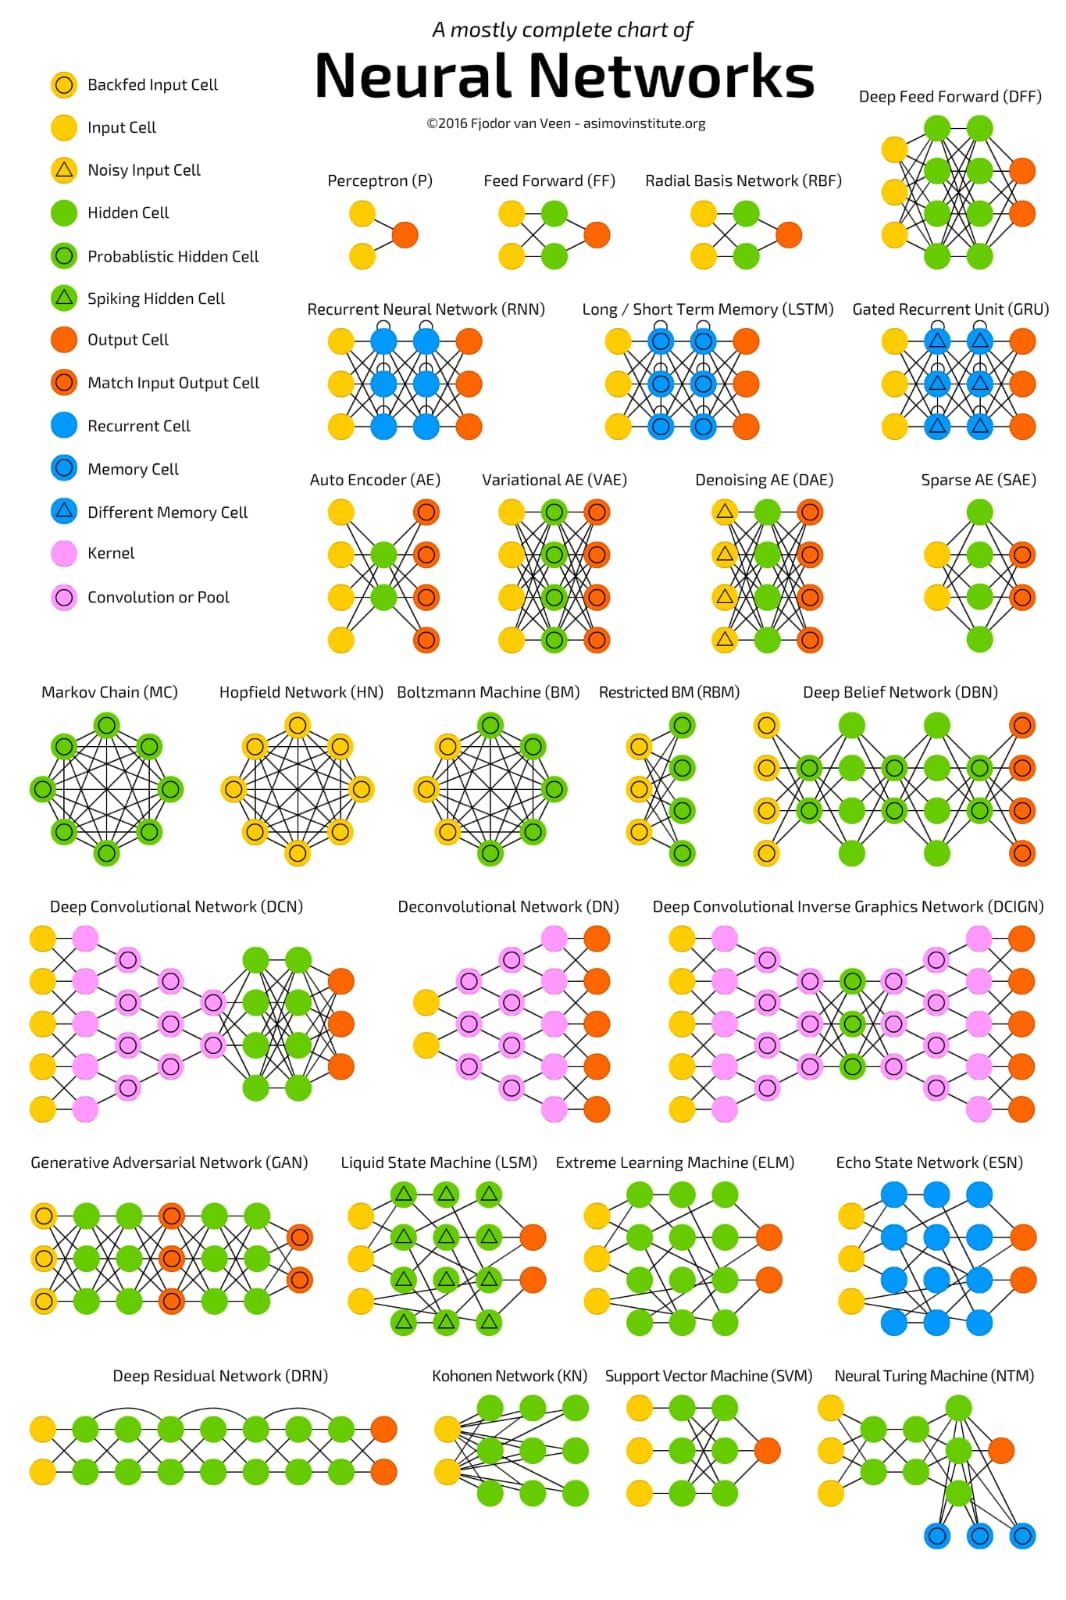
\includegraphics[width=0.9\textwidth]{imgs/neural_networks.jpeg}
  \caption{Panorama de arquiteturas de redes neurais \cite{asimov2017}}
  \label{fig:nnzoo}
\end{figure}

\FloatBarrier
\subsection{Large Language Models}

O funcionamento dos \textit{Large Language Models} (LLMs) envolve, inicialmente, uma fase de pré-treinamento sobre corpora textuais extensos e diversos. Nessa etapa, o modelo aprende representações estatísticas das palavras e suas relações contextuais. Subsequentemente, o modelo pode ser refinado por meio de técnicas de ajuste fino (\textit{fine-tuning}) para tarefas ou domínios específicos, como medicina, direito ou engenharia de software. Essa adaptação permite que o modelo adquira conhecimento especializado e aprimore seu desempenho em aplicações particulares \cite{jelodar2025, ouyang2023}.

Uma das características mais notáveis dos LLMs é sua capacidade de realizar generalização em tarefas para as quais não foram explicitamente programados. Isso ocorre porque, durante o treinamento, os modelos aprendem padrões sintáticos, semânticos e pragmáticos da linguagem, o que os capacita a inferir intenções, completar sentenças e até mesmo gerar respostas inéditas com base em instruções ambíguas ou vagas \cite{liu2024hallucinations, fan2023llmsw}.

Nesse sentido, no contexto da engenharia de software, os LLMs têm sido amplamente empregados para atividades como compreensão de requisitos, geração de código, documentação automatizada e verificação semântica. Tais aplicações se beneficiam da habilidade dos modelos em transitar entre linguagem natural e linguagem de programação, estabelecendo uma ponte entre a comunicação humana e a lógica computacional. Conforme apontado por \citeonline{jelodar2025}, o uso de LLMs em tarefas de análise de código tem-se mostrado promissor por sua capacidade de capturar estruturas semânticas profundas e apoiar a automação de tarefas críticas em ambientes de desenvolvimento.

Em suma, os LLMs representam um avanço significativo na interseção entre inteligência artificial e linguagem, oferecendo uma base tecnológica versátil para a construção de sistemas inteligentes capazes de compreender e manipular texto com sofisticação crescente.

\subsection{Arquitetura Transformer}

O avanço dos LLMs está intrinsecamente ligado à evolução de suas arquiteturas. Entre as diversas estruturas propostas, a arquitetura \textit{Transformer} representa um marco fundamental na história do processamento de linguagem natural, estabelecendo as bases dos modelos contemporâneos mais poderosos, como BERT, GPT e LaMDA.

A arquitetura Transformer foi projetada para resolver tarefas de transdução de sequência, como a tradução automática, de maneira mais eficiente que os modelos recorrentes anteriores, como RNNs e LSTMs. O elemento central do Transformer é o mecanismo de atenção, especialmente a \textit{self-attention}, que permite ao modelo capturar dependências contextuais entre quaisquer partes da entrada, independentemente de sua distância posicional, superando limitações comuns às redes recorrentes no aprendizado de relações de longo alcance no texto \cite{vaswani2017}.

A arquitetura original é composta por dois componentes principais: o codificador (\textit{encoder}) e o decodificador (\textit{decoder}). Ambos consistem em múltiplas camadas empilhadas, sendo que cada camada do codificador contém dois subcomponentes: um mecanismo de atenção multi-cabeça (\textit{multi-head attention}) e uma rede \textit{feedforward} totalmente conectada. O decodificador, por sua vez, incorpora um terceiro mecanismo de atenção, chamado \textit{encoder-decoder attention}, que permite integrar as representações aprendidas pelo codificador na geração das saídas \cite{ankit2024transformer}.  Essa estrutura pode ser visualizada na Figura~\ref{fig:transformer}, que ilustra a disposição dos principais componentes da arquitetura Transformer proposta por \citeonline{vaswani2017}

\begin{figure}[H]
    \centering
    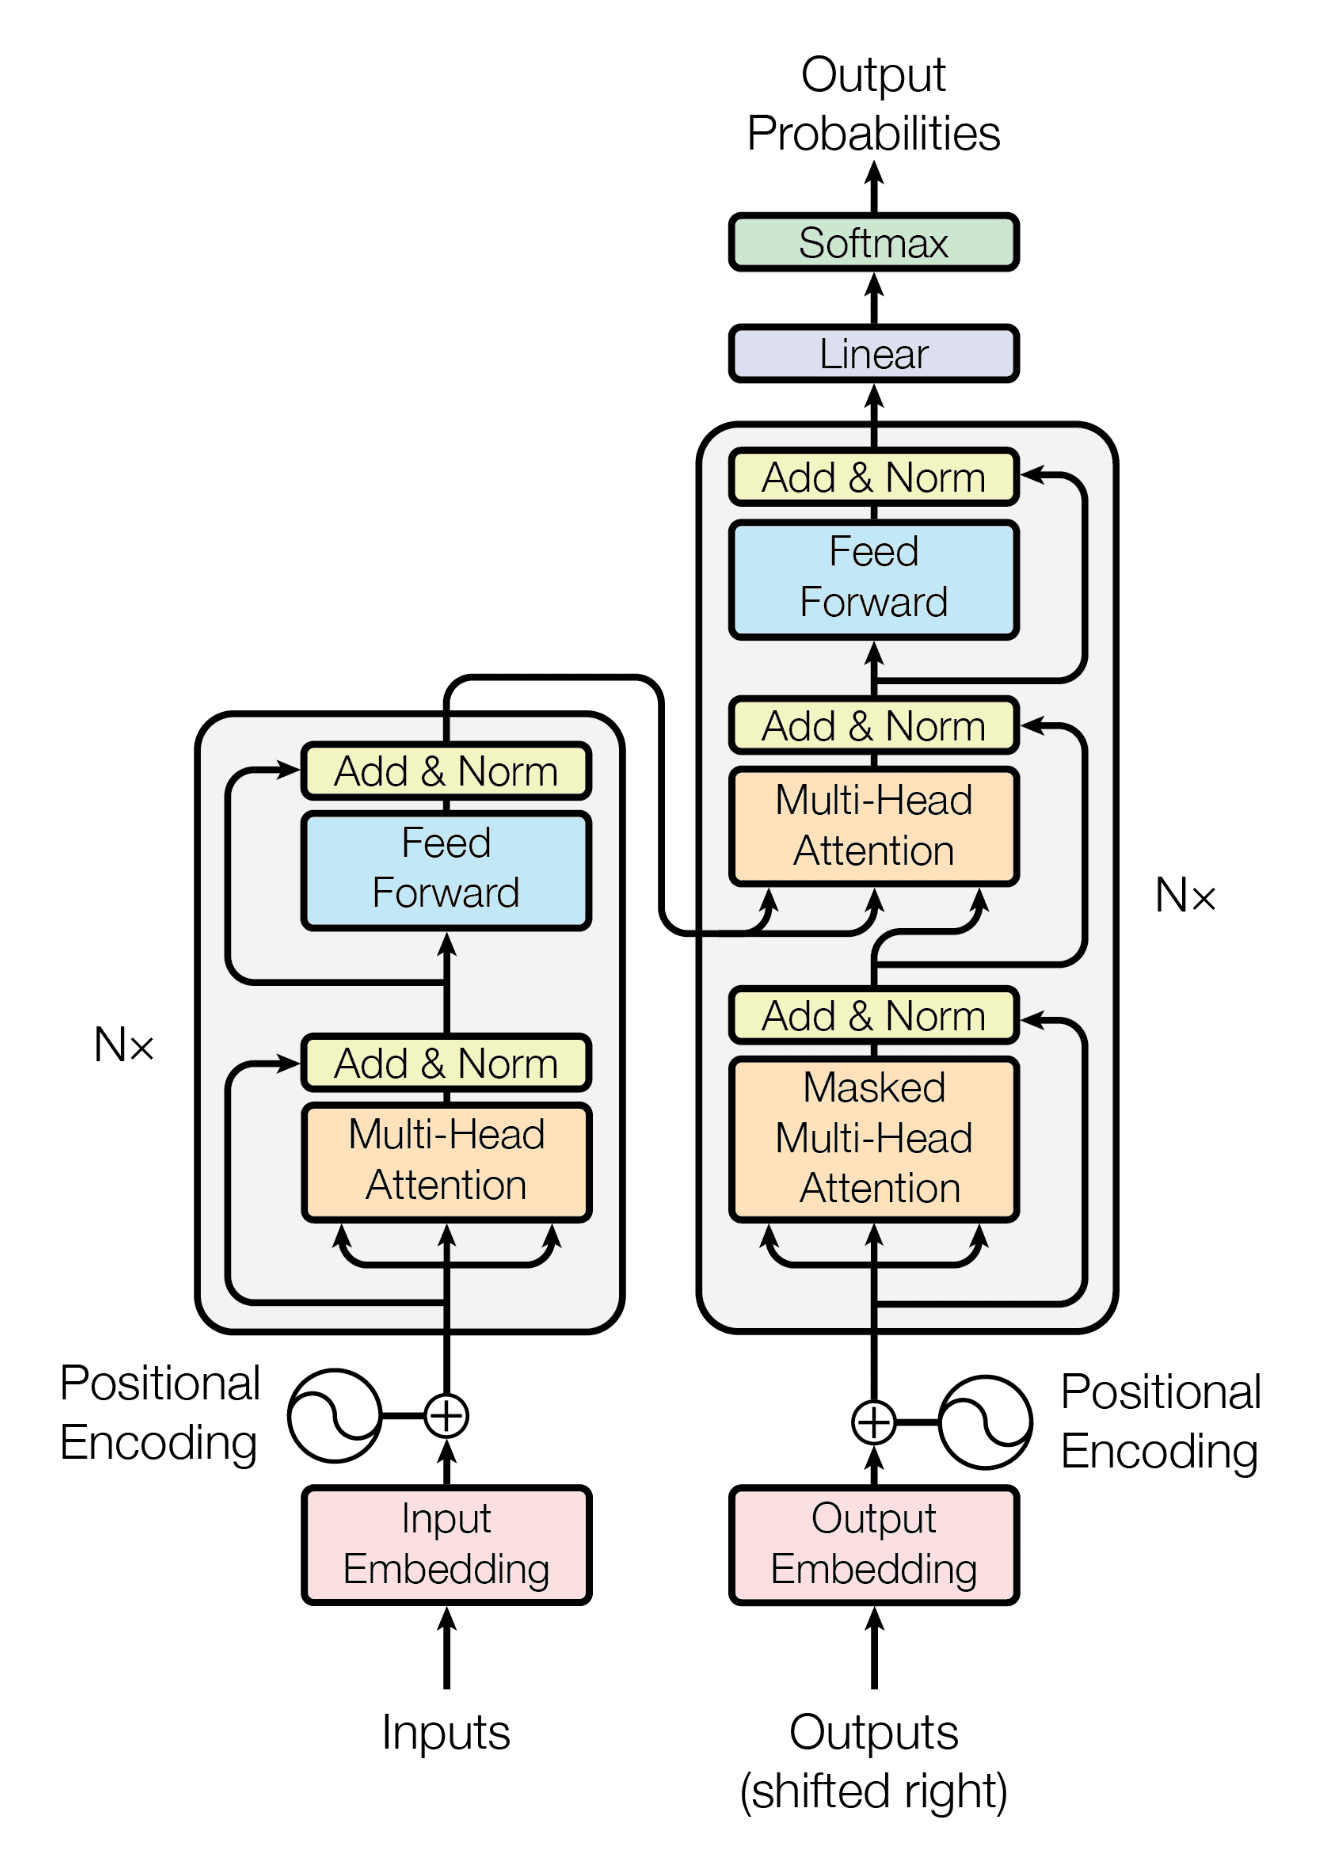
\includegraphics[width=0.75\textwidth]{imgs/transformer.png}
    \caption{Arquitetura do modelo Transformer \cite{vaswani2017}}
    \label{fig:transformer}
\end{figure}


Um dos aspectos mais inovadores do Transformer é a sua natureza altamente paralelizável, possibilitando ganhos significativos em desempenho computacional. Diferentemente das RNNs, que processam dados de forma sequencial, o Transformer permite o processamento simultâneo de todos os elementos da sequência de entrada, aproveitando de forma mais eficiente a arquitetura paralela das GPUs modernas \cite{ankit2024transformer}.

Para representar a ordem dos \textit{tokens} já que o modelo não possui uma estrutura sequencial intrínseca, são utilizados codificadores posicionais (\textit{positional encodings}), geralmente baseados em funções senoidais e cossenoidais de frequências variadas, os quais são somados aos vetores de \textit{embeddings} dos \textit{tokens} \citeonline{vaswani2017}. Essa codificação permite ao modelo inferir relações posicionais relativas entre os elementos da sequência.

Cada mecanismo de atenção da arquitetura é implementado por meio da chamada \textit{Scaled Dot-Product Attention}, onde o vetor de consulta (\textit{query}) é comparado com os vetores de chave (\textit{key}), e os resultados ponderam os vetores de valor (\textit{value}) para determinar a relevância contextual de cada \textit{token}. Esse processo é repetido em múltiplas cabeças de atenção (\textit{multi-head}), permitindo que o modelo aprenda diferentes aspectos das relações semânticas em paralelo \cite{ankit2024transformer, raschka2025bigllm}.

A partir da arquitetura original, diversas variantes e otimizações foram propostas. Modelos como GPT, BERT e T5 introduziram variações no uso do codificador, decodificador ou ambos, bem como aprimoramentos em camadas de normalização, mecanismos de atenção e escalabilidade. Além disso, técnicas como o uso de \textit{Mixture-of-Experts} (MoE), \textit{Grouped Query Attention} (GQA) e mecanismos de janela deslizante (\textit{sliding window attention}) foram desenvolvidas para aumentar a capacidade dos modelos e, ao mesmo tempo, reduzir os custos computacionais durante a inferência \citeonline{raschka2025bigllm}.

Esses avanços demonstram que, embora a estrutura base do Transformer permaneça amplamente utilizada, sua flexibilidade arquitetônica possibilitou diversas inovações. Atualmente, a arquitetura Transformer constitui a espinha dorsal da maioria dos LLMs de alto desempenho, permitindo não apenas avanços em tarefas linguísticas, mas também sua aplicação em domínios multimodais, como imagens, vídeos e interações conversacionais \cite{ankit2024transformer, raschka2025bigllm}.


\subsection{Janela de Contexto}

A janela de contexto de um modelo de linguagem representa a quantidade de informações textuais que o modelo é capaz de processar simultaneamente. Trata-se de um parâmetro crucial para tarefas que envolvem raciocínio sobre longos documentos, como verificação de requisitos em código-fonte, sumarização e busca semântica. O tamanho e o funcionamento da janela de contexto têm implicações diretas na eficácia e nas limitações dos modelos de linguagem natural, particularmente os baseados na arquitetura Transformer.

O modelo Transformer, proposto por \citeonline{vaswani2017}, introduziu o mecanismo de autoatenção como forma de modelar dependências globais entre \textit{tokens} sem recorrer a estruturas sequenciais como RNNs. Cada \textit{token} pode se conectar com qualquer outro \textit{token} da sequência por meio de uma matriz de atenção, o que implica em uma complexidade quadrática em relação ao tamanho da entrada. Embora isso permita modelar dependências de longo alcance com eficiência teórica, o custo computacional impõe limites práticos ao comprimento da janela de contexto suportada.

Para contornar essa limitação, estratégias como o \textit{chunking} (divisão de textos em segmentos menores) passaram a ser adotadas em sistemas de Recuperação Aumentada por Geração (RAG). Contudo, o \textit{chunking} tradicional, no qual os trechos são vetorizados separadamente, pode causar a perda de contexto semântico. Para enfrentar esse desafio, \citeonline{gunther2025} propuseram o método \textit{Late Chunking}, que primeiro vetoriza todo o documento com modelos de contexto longo e, só depois, aplica o agrupamento para o cálculo das representações vetoriais dos \textit{chunks}. Isso permite que os vetores reflitam a semântica global do documento, superando a limitação contextual dos métodos tradicionais.

Além disso, \citeonline{jin2024} propuseram o método \textit{SelfExtend}, que demonstra que modelos com codificações posicionais relativas, como RoPE, possuem capacidades inatas para processar sequências mais longas do que aquelas observadas durante o treinamento. A técnica consiste em modificar a atenção de forma que posições relativas fora da distribuição original sejam mapeadas para valores já observados, estendendo efetivamente a janela de contexto sem necessidade de \textit{fine-tuning}. Isto é especialmente relevante para tarefas que requerem consistência contextual em documentos extensos, como a análise de requisitos de software dispersos em arquivos distintos.

Ambas as abordagens mostram que a eficácia do modelo diante de textos longos depende não apenas do tamanho da janela de contexto, mas também da forma como a informação contextual é preservada e utilizada na geração dos \textit{embeddings}. Neste sentido, métodos como \textit{Late Chunking} e \textit{SelfExtend} tornam-se particularmente promissores para aplicações em que a rastreabilidade e a fidelidade semântica ao longo do texto são essenciais.

Por fim, destaca-se que o aproveitamento eficiente da janela de contexto é diretamente influenciado pelo design da arquitetura, pelas estratégias de vetorização e pela engenharia de \textit{prompts}. Assim, o estudo da janela de contexto é um componente fundamental para compreender os limites e as possibilidades dos modelos de linguagem em tarefas que envolvem grandes volumes de informação textual.

\subsection{Funcionamento e Parâmetros dos Modelos de Linguagem}

Os LLMs funcionam por meio de um processo dividido em duas fases: treinamento e geração. Na fase de treinamento, o modelo é exposto a grandes volumes de dados textuais e ajusta internamente seus parâmetros para aprender padrões linguísticos, sintáticos e semânticos. O número de parâmetros varia conforme o modelo, podendo atingir centenas de bilhões ou até trilhões, como é o caso do GPT-4, que apresenta arquitetura do tipo \textit{mixture-of-experts} com cerca de 1,8 trilhão de parâmetros \citeonline{openai2023}. Esses parâmetros são responsáveis por representar o conhecimento aprendido e são fixados após o treinamento. Na fase de inferência, por sua vez, o comportamento do modelo passa a ser governado por hiperparâmetros que controlam como as respostas são geradas a partir desse conhecimento prévio.

Entre esses hiperparâmetros, destaca-se a \textit{temperature}, que regula o grau de aleatoriedade da geração textual. Em termos práticos, valores baixos de \textit{temperature} (próximos de 0) resultam em respostas mais determinísticas, favorecendo a exatidão e a repetição de padrões aprendidos; por outro lado, valores mais altos (acima de 1.0) promovem maior diversidade e imprevisibilidade na escolha dos \textit{tokens} subsequentes. A configuração apropriada desse parâmetro é especialmente relevante em contextos técnicos, como a análise de requisitos de software, nos quais a fidelidade semântica e a consistência textual são essenciais \citeonline{renze2024}.

Outros parâmetros amplamente utilizados incluem o \textit{top-k} e o \textit{top-p}. O \textit{top-k} restringe a escolha do próximo \textit{token} aos `k` \textit{tokens} mais prováveis, limitando o espaço de amostragem e eliminando opções de baixa probabilidade, o que favorece a coesão em tarefas com vocabulário mais técnico ou padronizado \citeonline{holtzman2020}. O \textit{top-p}, também conhecido como \textit{nucleus sampling}, adota uma abordagem dinâmica ao selecionar o menor conjunto de \textit{tokens} cuja soma de probabilidades atinja um limite cumulativo (geralmente entre 0,8 e 0,95), permitindo um equilíbrio entre variedade e controle estatístico da geração \citeonline{fan2018}.

Além disso, penalidades de frequência e de presença são utilizadas para mitigar repetições, incentivando o uso de vocabulário mais diverso em textos extensos. Estas penalidades reduzem a probabilidade de reaparecimento de \textit{tokens} já utilizados, sendo particularmente úteis em aplicações que envolvem geração de documentação técnica, explicações ou justificativas complexas \citeonline{openai2023}.

A interação entre esses hiperparâmetros permite a adaptação do comportamento do modelo às necessidades específicas de diferentes tarefas. Por exemplo, na verificação automatizada de requisitos, recomenda-se utilizar \textit{temperature} baixa e \textit{top-p} moderado, a fim de priorizar a exatidão e reduzir alucinações. Já em tarefas de geração descritiva ou criativa, como a escrita de histórias de usuários ou a geração de testes automatizados com descrições narrativas, configurações mais permissivas favorecem a variabilidade sem comprometer a utilidade \citeonline{raffel2020}.

Embora tradicionalmente se associe a \textit{temperature} ao controle da “criatividade” de um modelo, estudos recentes indicam que sua influência é limitada em comparação com outros fatores, como a estrutura da tarefa ou o tipo de \textit{fine-tuning} aplicado \citeonline{nguyen2025}. Isso reforça a necessidade de compreender esses parâmetros como elementos que interagem entre si, exigindo ajustes experimentais cuidadosos conforme o domínio de aplicação.

Dessa forma, os parâmetros de decodificação exercem papel central na fase de inferência dos modelos de linguagem, moldando o estilo, a coerência e a adequação da saída gerada. No contexto de engenharia de software, em especial na análise de conformidade de requisitos, sua correta configuração é essencial para garantir não apenas a relevância da resposta, mas também a rastreabilidade semântica e a consistência técnica com os artefatos analisados.

\subsection{Embedding, Chunk e Vetorização}

O uso de \textit{embeddings} vetoriais tem se consolidado como uma abordagem essencial no processamento de linguagem natural (PLN), especialmente no contexto de LLMs. A técnica consiste na transformação de dados textuais não estruturados em vetores de alta dimensionalidade que capturam semântica e contexto, permitindo que sistemas computacionais realizem tarefas como busca semântica, recuperação de informações e verificação de similaridade com maior eficiência \citeonline{lema2025}.

O processo de vetorização normalmente se inicia com a fragmentação do conteúdo textual em segmentos menores, denominados \textit{chunks}. Esses \textit{chunks} são projetados para respeitar os limites da janela de contexto do modelo, otimizando a capacidade de raciocínio e minimizando a perda de informação semântica. A definição do tamanho do \textit{chunk} deve equilibrar a granularidade da análise e a eficiência da indexação, sendo comum a adoção de janelas de 512 a 1024 \textit{tokens} em aplicações práticas \citeonline{muennighoff2022}.

Uma vez definidos, os \textit{chunks} são processados por modelos de \textit{embedding}, os quais produzem representações vetoriais que preservam relações semânticas e sintáticas entre os textos originais. No caso do SGPT, por exemplo, é aplicada uma técnica de \textit{weighted mean pooling} sobre os estados ocultos dos \textit{tokens}, ponderando a influência de \textit{tokens} mais à frente na sequência, uma vez que o modelo é baseado em atenção causal \citeonline{muennighoff2022}. Esta abordagem demonstrou superioridade em tarefas de busca semântica simétrica e assimétrica, com ganhos de desempenho notáveis quando comparados a \textit{embeddings} tradicionais.

Após a geração dos \textit{embeddings}, esses vetores são armazenados em bases de dados vetoriais (\textit{Vector Databases} – VDBs), que viabilizam operações de similaridade por meio de técnicas de busca aproximada ao vizinho mais próximo (\textit{Approximate Nearest Neighbor Search} – ANNS). Tais técnicas utilizam estruturas como índices hierárquicos, árvores k-d, grafos navegáveis e particionamentos baseados em quantização para permitir a recuperação eficiente mesmo em cenários de altíssima dimensionalidade \citeonline{lema2025}. Essa arquitetura é particularmente relevante para aplicações que requerem resposta em tempo real ou processamento em larga escala, como nos sistemas de Recuperação Aumentada por Geração (RAG) empregados em soluções corporativas e agentes autônomos.

A eficácia do processo de vetorização não depende apenas do modelo utilizado para gerar os \textit{embeddings}, mas também de boas práticas no pré-processamento textual, como a remoção de ruídos e a padronização da linguagem. Além disso, a forma como os \textit{chunks} são segmentados influencia diretamente na manutenção do contexto e da coerência semântica ao longo dos vetores gerados \citeonline{muennighoff2022}. Outro aspecto importante é a aplicação de técnicas de normalização nos vetores, como a normalização L2, que garante que as métricas de similaridade permaneçam matematicamente consistentes e comparáveis em grandes volumes de dados \citeonline{lema2025}.

A integração dessas tecnologias tem permitido o desenvolvimento de sistemas inteligentes capazes de realizar busca semântica de alta precisão, detecção de duplicidade textual, verificação de conformidade entre requisitos e código-fonte, bem como sumarização e rastreabilidade de informações em \textit{pipelines} automatizados de engenharia de software.

\subsection{Engenharia de Prompt e Protocolo MCP}

A engenharia de \textit{prompt} tem emergido como uma prática central na interação com LLMs, sendo especialmente relevante em contextos empresariais e acadêmicos. Essa técnica consiste na formulação de instruções textuais com o objetivo de elicitar comportamentos específicos dos modelos, como sumarização, classificação, geração de código e análise de documentos. \citeonline{desmond2024} destacam que, embora o uso de linguagem natural sugira uma interação intuitiva, a construção de \textit{prompts} eficazes exige conhecimento técnico, compreensão do funcionamento interno dos modelos e uma abordagem iterativa.

Estudos conduzidos por \citeonline{kin2023} apontam que usuários frequentemente cometem erros conceituais ao tentar interagir com LLMs, o que evidencia a necessidade de ferramentas e metodologias que auxiliem na criação de \textit{prompts} mais robustos. Complementarmente, \citeonline{braun2024} propõem uma taxonomia dos componentes do \textit{prompt}, destacando a importância do refinamento das instruções e da adaptação do conteúdo contextual.

Pesquisas empíricas demonstram que usuários experientes costumam ajustar elementos do \textit{prompt} como a instrução da tarefa, o contexto fornecido e o formato esperado da resposta. De acordo com \citeonline{desmond2024}, as alterações mais frequentes incluem modificações semânticas, adição de exemplos e reestruturações de formato. Além disso, estratégias avançadas têm se mostrado eficazes em tarefas complexas, como o \textit{few-shot prompting}, que consiste em fornecer alguns exemplos da tarefa desejada para guiar o modelo, e o \textit{chain-of-thought}. Esta última técnica é definida pelo "encadeamento de raciocínio" no \textit{prompt}, o que, segundo \citeonline{wei2022}, auxilia na execução de tarefas que requerem múltiplas etapas cognitivas. Em outra abordagem, \citeonline{melamed2023} tratam o design de \textit{prompts} como um problema inverso, propondo modelos que otimizam automaticamente sua estrutura para maximizar a performance.

A complexidade da engenharia de \textit{prompt} aumenta quando se busca garantir rastreabilidade entre os requisitos expressos em linguagem natural e os artefatos de software correspondentes. Nesse contexto, destaca-se o uso do \textit{Model Context Protocol} (MCP) como um mecanismo padronizado que organiza a comunicação entre modelos de linguagem e sistemas externos. O MCP opera em uma arquitetura cliente-servidor, onde aplicações de IA (\textit{hosts}) se conectam a servidores MCP especializados para obter dados contextuais relevantes. Esses servidores podem disponibilizar ferramentas, recursos e \textit{prompts} estruturados, que são acessados dinamicamente pelos modelos durante a execução de tarefas.

O protocolo é dividido em duas camadas principais: a camada de dados, baseada em JSON-RPC 2.0, que define como tarefas, respostas e recursos são trocados; e a camada de transporte, responsável pela conexão e autenticação, que pode funcionar via STDIO para servidores locais ou HTTP para servidores remotos \citeonline{mcp2024}.

Ao integrar a engenharia de \textit{prompt} com o MCP, é possível criar fluxos interativos e auditáveis nos quais os modelos obtêm contexto em tempo real, executam ferramentas externas ou acessam bases de conhecimento estruturadas com alta rastreabilidade. Essa abordagem fortalece a confiabilidade das LLMs em tarefas críticas, como análise de requisitos de software, verificação de conformidade e geração automatizada de artefatos técnicos.


\subsection{Agentes de Inteligência Artificial}


Agentes de Inteligência Artificial (IA) são entidades autônomas de software projetadas para executar tarefas específicas de forma adaptativa, racional e contínua. Fundamentados em ciclos de percepção, raciocínio e ação, esses agentes analisam entradas do ambiente (digitais ou físicos), tomam decisões com base em regras, heurísticas ou modelos treinados, e atuam para atingir metas estabelecidas. Diferentemente de assistentes baseados apenas em prompts ou scripts determinísticos, os agentes de IA modernos possuem certo grau de autonomia operacional, podendo interagir com APIs, sistemas de arquivos, modelos de linguagem e bancos de dados (IBM, 2024; AWS, 2024).

Com o avanço dos modelos fundacionais, especialmente os LLMs, esses agentes passaram a incorporar mecanismos de raciocínio natural, recuperação semântica e execução contextualizada de comandos. Isso os torna aptos a realizar tarefas como responder perguntas, sintetizar documentos, realizar buscas, chamar funções externas, interpretar imagens, gerar relatórios ou interagir com sistemas complexos de forma autônoma (Sapkota et al., 2025). Aplicações práticas incluem assistentes corporativos inteligentes, bots de atendimento, análise automatizada de requisitos de software e agentes robóticos embarcados. Empresas como AWS, Google, IBM e Microsoft já adotam arquiteturas baseadas em agentes para orquestração de tarefas entre serviços internos e externos.

A IBM (2024) propõe uma arquitetura modular baseada em três elementos principais: um plano de raciocínio e tomada de decisão; um componente de memória para estado e contexto; e um executor que interage com ferramentas, sistemas e APIs. Essa estrutura permite que o agente seja continuamente invocado por eventos, mantenha persistência sobre tarefas anteriores e adapte seu comportamento a partir do histórico. Além disso, agentes podem ser organizados em sistemas cooperativos, uma abordagem conhecida como Agentic AI  em que múltiplos agentes especializados trabalham de forma coordenada para resolver problemas complexos, com divisão de tarefas, comunicação entre agentes e reuso de memória compartilhada (Sapkota et al., 2025).

O conceito de Agentic AI amplia a atuação dos agentes convencionais ao introduzir estruturas colaborativas compostas por unidades autônomas com papéis distintos. Tais agentes são capazes de operar em camadas distintas, como planejadores, executores ou verificadores, interagindo entre si para atingir metas coletivas de forma eficaz. Ferramentas como AutoGen, CrewAI e LangGraph já exploram esse paradigma, permitindo a criação de pipelines autônomos, fluxos de raciocínio distribuído e agentes capazes de coordenar ações em ambientes híbridos físicos-digitais com alto grau de adaptabilidade (Sapkota et al., 2025).
